\documentclass[preprint]{aastex631}
\usepackage{graphicx}
\usepackage{natbib}
\bibliographystyle{aasjournal}

\begin{document}

\title{An example \LaTeX\ report}

\author{Bradford A. Benson}
\affil{Department of Astronomy \& Astrophysics, University of Chicago}

\begin{abstract}
The abstract is a short paragraph which summarizes your paper / lab report / etc. It has to state what you did, what your results are, and your conclusions.  It is not an introduction, and it should not state anything that is not found in the main text, as well.
\end{abstract}

\section{Introduction}

Make sure you cite the appropriate literature references.  To do so, look up each paper on ADS\footnote{http://adswww.harvard.edu/abstract\_service.html} and click on ``Bibtex entry for this abstract''.  Copy the text starting at ``\@'' and ending with the closing ``\}'' into a separate text file such as ``references.bib''.  You will probably want to change the identifier, which is the string between the first ``\{'' and the first comma, to something easy to remember.  This identifier is used to reference the paper in the text using ``citet'' or ``citep'', as appropriate: \citet{dibert21} for in-line vs. \citep{guns21} in parentheses.  See the conclusion of this text for how to compile the document with this structure.

\section{A Section}

\subsection{A sub-section}

\subsubsection{A sub-sub-section}

\section{Images}

The images that you include should either all be {\tt .eps} files (encapsulated post-script), or a mix of {\tt .pdf} and {\tt .jpg} files.  The {\tt graphicx} package is a common and versatile way of including figures.

\begin{figure}[htb]
\begin{center}
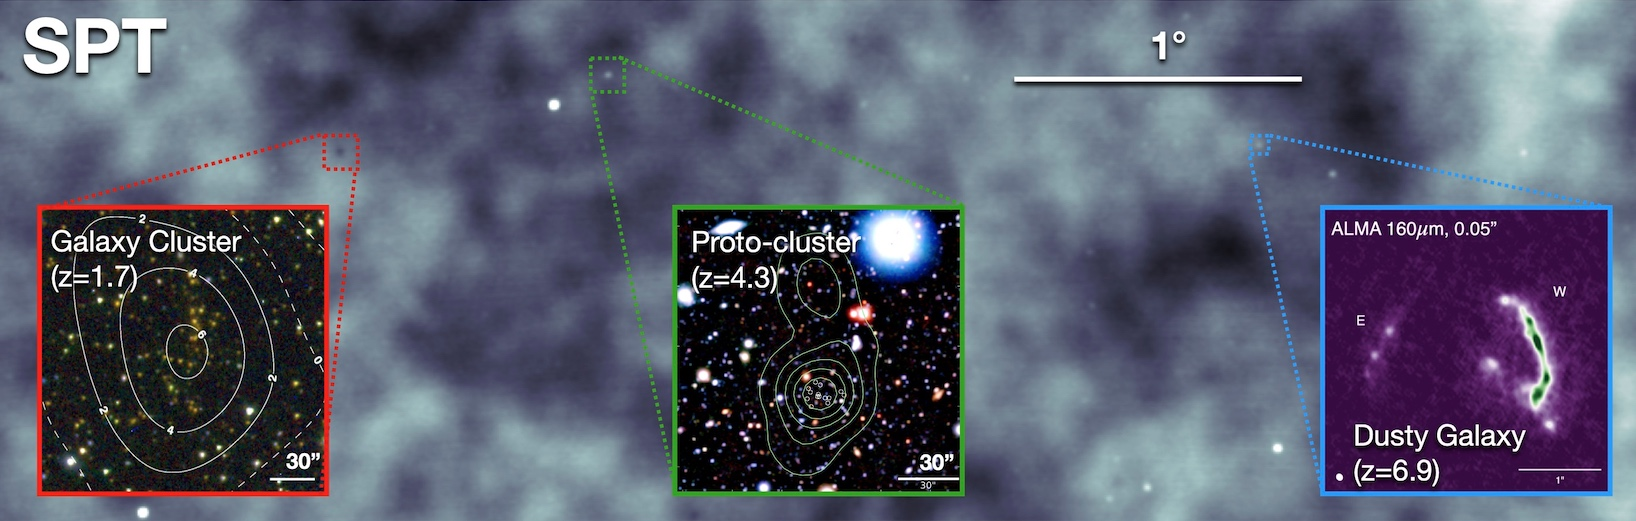
\includegraphics[width=0.85\hsize]{2021_01_SPT_maps_sources_v2.jpg}
\caption{An example of a jpg figure.}
\label{fig:spt_gallery}
\end{center}
\end{figure}

Note that this figure is defined as a ``float''.  \LaTeX\ will automatically place it where it fits best.  Since we have given the figure a label, you can reference the figure as Fig.~\ref{fig:spt_gallery}.

\section{Tables}

Tables are produced with the {\tt tabular} environment and can also be placed inside floats.  The are labeled and referenced just like figures, e.g. in this case we have Table~\ref{tab:observations}

\begin{table}[htb]
\caption{Note that for tables, the caption comes before the table.}
\label{tab:observations}
\begin{center}
\begin{tabular}{p{2.0in}rcrc}
%\multicolumn{5}{c}{TABLE 1} \\
\multicolumn{5}{c}{Journal of Observations} \\
\tableline
\tableline
& \multicolumn{1}{c}{Date of} & & \multicolumn{1}{c}{Exposure} &
\multicolumn{1}{c}{Limiting} \\
\multicolumn{1}{c}{Object} & \multicolumn{1}{c}{Observation} &
\multicolumn{1}{c}{Filter} & \multicolumn{1}{c}{Time} (s) &
\multicolumn{1}{c}{Magnitude} \\
\tableline
Object 1 \dotfill & Jan 1, 2022 & {\em U} & 1000 & 20.0 \\
& Jan 1, 2022 & {\em B} & 500 & 20.1 \\
& Jan 1, 2022 & {\em V} & 300 & 20.2 \\
Object 2 \dotfill & Feb 2, 2022 & {\em U} & 2000 & 20.3 \\
& Feb 2, 2022 & {\em B} & 1000 & 20.3 \\
Object 3\tablenotemark{a} \dotfill & Mar 3, 2022 & {\em U} & 1000 & 19.0 \\
& Mar 3, 2022 & {\em V} & 500 & 19.5 \\
\tableline
\end{tabular}
\tablenotetext{a}{Tables can contain footnotes.}
\end{center}
\end{table}

\section{Equations}

\LaTeX\  was built for convenient type-setting of mathematical equations:
\begin{equation}
\mu = \frac{1}{N} \sum_{i = 1}^N x_i
\end{equation}
and
\begin{equation}
\sigma_\mu^2 = \frac{1}{N-1} \sum_{i = 1}^N (x_i - \mu)^2.
\label{eq:std-dev}
\end{equation}
And you can also label and reference them, such as Eq.~\ref{eq:std-dev}.

\section{Compiling your document}

If you use labels for figures, tables, and equations in the text, you have compile your document twice.  When using BibTeX, as we are here, you even have to compile it three times, as well as add a call to BibTeX after the first time.  How you compile it depends on what type of figures you are using.  If you are using {\tt .eps} files, you compile with {\tt latex}, otherwise it is easiest to use {\tt pdflatex}.  This example document document would be compiled using:

\noindent{\tt
pdflatex example.tex\\
bibtex example\\
pdflatex example.tex\\
pdflatex example.tex
}

\bibliography{references}

\end{document}
